\section{Adaptación}\label{sec:adaptacion}
La adaptación de textos es un proceso de transformación lingüística que busca ajustar la dificultad de un contenido escrito para satisfacer las necesidades de un público objetivo específico. En el ámbito del procesamiento de lenguaje natural (NLP), esta tarea se aborda tradicionalmente desde dos vertientes: la simplificación de textos (Text Simplification, TS), que reduce la complejidad léxica y sintáctica, y la complejización, que busca enriquecer el texto para desafiar a lectores con competencias más avanzadas.

Aunque la adaptación es bidireccional, la vasta mayoría de la literatura y los esfuerzos de investigación se han concentrado en la simplificación. Históricamente, el objetivo principal de la TS ha sido mejorar la accesibilidad para lectores con bajos niveles de alfabetización o desafíos cognitivos (Siddharthan, 2014)[cita]. Sin embargo, en el contexto de la enseñanza de lenguas extranjeras, surge un requisito adicional y más restrictivo: la simplificación controlada por niveles de suficiencia (Readability-Controlled Text Simplification o RCTS).

En este trabajo, el enfoque se centra exclusivamente en la simplificación de textos, entendida como la capacidad de transformar un material de entrada de alta complejidad hacia niveles inferiores de la escala CEFR. Esta necesidad ha sido recientemente validada por iniciativas internacionales como la shared task TSAR 2025 (Alva-Manchego et al., 2025)[cita], la cual propone simplificar textos de niveles B2 o superiores hacia niveles específicos como A2 o B1. Bajo esta premisa, nuestra investigación no solo busca reducir la complejidad general, sino garantizar que el texto resultante sea pedagógicamente adecuado para el estadio de aprendizaje del estudiante, preservando estrictamente el significado y la coherencia del mensaje original.

\subsection{Trabajo relacionado}\label{subsection:ad_trabajo}
La tarea de adaptación de textos se apoya sobre dos pilares fundamentales que han sido objeto de estudio intenso en la literatura de PLN: la evaluación automática de legibilidad (ARA) y la simplificación de textos (TS). En esta sección revisamos la evolución de ambas áreas, con especial énfasis en los enfoques que incorporan control explícito sobre el nivel objetivo, conocidos como Readability-Controlled Text Simplification (RCTS), dado que constituyen el antecedente más directo del trabajo presentado en este capítulo.
\subsubsection{Evaluación automática de legibilidad (ARA)}
Como se introdujo en el capítulo de clasificación (\Cref{subsection:clas_trabajo}), la ARA busca modelar la dificultad de lectura y comprensión de un texto para una audiencia determinada \cite{Feng2010}. Su relevancia para la adaptación es doble: por un lado, permite caracterizar el nivel de un texto de entrada antes de transformarlo; por otro, sirve como criterio de validación para verificar que el texto generado haya alcanzado el nivel objetivo.
Las fórmulas tradicionales, como Flesch-Kincaid \cite{Kincaid1975} o SMOG \cite{smog}, fueron los primeros instrumentos utilizados para este fin. Sin embargo, su capacidad de capturar la complejidad real de un texto es limitada, ya que no consideran aspectos semánticos ni discursivos que resultan centrales para juzgar si una adaptación es pedagógicamente adecuada para un estudiante L2. Trabajos posteriores incorporaron características lingüísticas más ricas y modelos de aprendizaje automático \cite{Xia2019}, mejorando la sensibilidad del sistema ante variaciones sutiles de complejidad, lo que resulta especialmente relevante cuando se evalúan adaptaciones entre niveles adyacentes del CEFR.
\subsubsection{Simplificación de textos (TS)}
La simplificación de textos busca transformar un documento en una versión de menor complejidad léxica y sintáctica, preservando su contenido informativo. Los enfoques iniciales fueron basados en reglas o métodos estadísticos. Con la llegada de los modelos neuronales, la calidad de las simplificaciones mejoró sustancialmente, permitiendo realizar operaciones de reescritura más naturales y coherentes.
Con el surgimiento de los LLMs, la investigación en TS se ha desplazado hacia el ajuste fino y la ingeniería de prompts, lo que ha reducido la dependencia de corpus paralelos de gran tamaño y ha abierto la posibilidad de adaptar el sistema a distintos dominios y audiencias con menor esfuerzo de anotación.
\subsubsection{Simplificación controlada por nivel de legibilidad (RCTS)}
La RCTS extiende la TS introduciendo un control explícito sobre el nivel de dificultad del texto resultante. Esto la hace especialmente valiosa en contextos educativos, donde no basta con simplificar, sino que es necesario garantizar que el texto generado sea adecuado para un perfil concreto de estudiante. La mayoría de los trabajos en esta área han seguido enfoques de entrenamiento supervisado, apoyándose en corpus paralelos donde cada par de textos contiene el original y su versión adaptada a un nivel objetivo. La principal limitación de esta estrategia es la escasez de datos disponibles, un problema que se agudiza cuando se trabaja con la escala CEFR, dado que los corpus de pares de adaptaciones alineadas a niveles específicos son prácticamente inexistentes para el inglés como L2.
Frente a esta limitación, los avances recientes en LLMs han abierto nuevas direcciones para la RCTS, explorando tanto la simplificación a nivel de oración como a nivel de pasaje completo, en configuraciones de zero-shot y few-shot. Estos trabajos muestran resultados prometedores en cuanto a la capacidad de los modelos para respetar el nivel objetivo sin necesidad de entrenamiento específico, aunque también evidencian limitaciones en la preservación del significado y en la consistencia de las adaptaciones, especialmente cuando se trabaja con niveles del CEFR muy distantes entre sí.
En este trabajo nos posicionamos en esta línea de investigación, abordando la RCTS a nivel de documento completo y evaluando el desempeño de LLMs open-source mediante distintas estrategias de prompting, con el objetivo de determinar en qué medida estos modelos son capaces de producir adaptaciones pedagógicamente adecuadas para estudiantes de inglés como segunda lengua.

\subsection{Diseño de Experimentos}\label{subsection:ad_diseño}
El objetivo de esta sección es describir el diseño experimental utilizado para evaluar la capacidad de LLMs en la tarea de adaptación de textos según los niveles del CEFR. A diferencia de la clasificación, donde la salida esperada es una etiqueta discreta, la adaptación requiere generar un texto completo que satisfaga simultáneamente múltiples criterios: adecuación al nivel objetivo, preservación del significado del texto original y coherencia lingüística. Esta mayor complejidad motivó un diseño experimental que combina distintas estrategias de prompting, procedimientos de refinamiento iterativo y un mecanismo de selección por votación.

\subsubsection{Selección del modelo}
A diferencia del capítulo de clasificación, donde se compararon múltiples modelos open-source y privativos, en los experimentos de adaptación se optó por trabajar exclusivamente con el modelo Meta-Llama-3.1-8B-Instruct. Esta decisión se fundamenta en tres razones: (i) su carácter open-source y bajo costo computacional relativo; (ii) su buen desempeño en la tarea de clasificación CEFR documentado en el capítulo anterior; y (iii) evidencia previa en la literatura de que modelos de la familia Llama 3 8B han demostrado ser efectivos en tareas similares de simplificación controlada. El modelo fue ejecutado con precisión bfloat16 y los parámetros de decodificación por defecto detallados en el \Cref{sec:parametros}.

\subsubsection{Tipos de prompting}
Se diseñaron y evaluaron de manera sistemática diez prompts distintos que se encuentran [cita], agrupados en dos tipos principales que representan 2 niveles de complejidad distintos:

\begin{itemize}

  \item \textbf{Prompting directo con información lingüística (few-shot)}
  Se construyó una serie de prompts extensos que incorporan información lingüística explícita sobre el nivel CEFR objetivo. Esta información incluye: (i) descriptores generales de comprensión lectora del CEFR para los niveles A2 y B1; (ii) listas de vocabulario frecuente y relevante para cada nivel, obtenidas de recursos de Oxford University Press; y (iii) ejemplos de construcciones morfosintácticas características de cada nivel. Adicionalmente, el prompt incorpora pares de ejemplos de textos originales y sus adaptaciones correspondientes, y contiene instrucciones explícitas para que el modelo produzca únicamente el texto adaptado, sin incluir meta-información sobre la tarea realizada.

  Si bien este tipo de prompt es el más informativo, su principal limitación es la longitud resultante, que supera los 3.800 tokens en promedio, lo cual puede afectar negativamente el desempeño del modelo por efectos de saturación de contexto, tal como se observó en los experimentos de clasificación.

  \item \textbf{Procedimientos de refinamiento iterativo (multi-step)}
  Para abordar la tensión entre la adecuación al nivel CEFR y la preservación del contenido original, se exploraron estrategias de dos pasos. En una primera variante, tras obtener una adaptación inicial con el prompt extenso, se aplica un segundo prompt orientado exclusivamente a la preservación del contenido, priorizando la fidelidad semántica sobre la adecuación lingüística al nivel. En una segunda variante, el segundo paso se destina a eliminar la meta-información producida por el modelo, referencias explícitas al nivel CEFR o a la tarea de simplificación, que aparece frecuentemente en las salidas a pesar de que el prompt la prohibe explícitamente.

\end{itemize}

\Cref{fig:grafico_tokens_adaptacion} presenta el número de tokens por prompt, revelando una gran diferencia de longitud entre los diseños propuestos. Es crucial tener en cuenta que el valor reportado en el gráfico corresponde únicamente al largo fijo del prompt (instrucciones y ejemplos). Por lo tanto, el contexto total para un prompt de tipo few-shot (barras azules) es la suma del prompt y el texto original. En contraste, para el refinamiento iterativo (barras verdes), la longitud total operativa se compone de la suma del prompt, el texto original y la adaptación preliminar generada en el primer paso.

\begin{figure}[H]
  \centering
  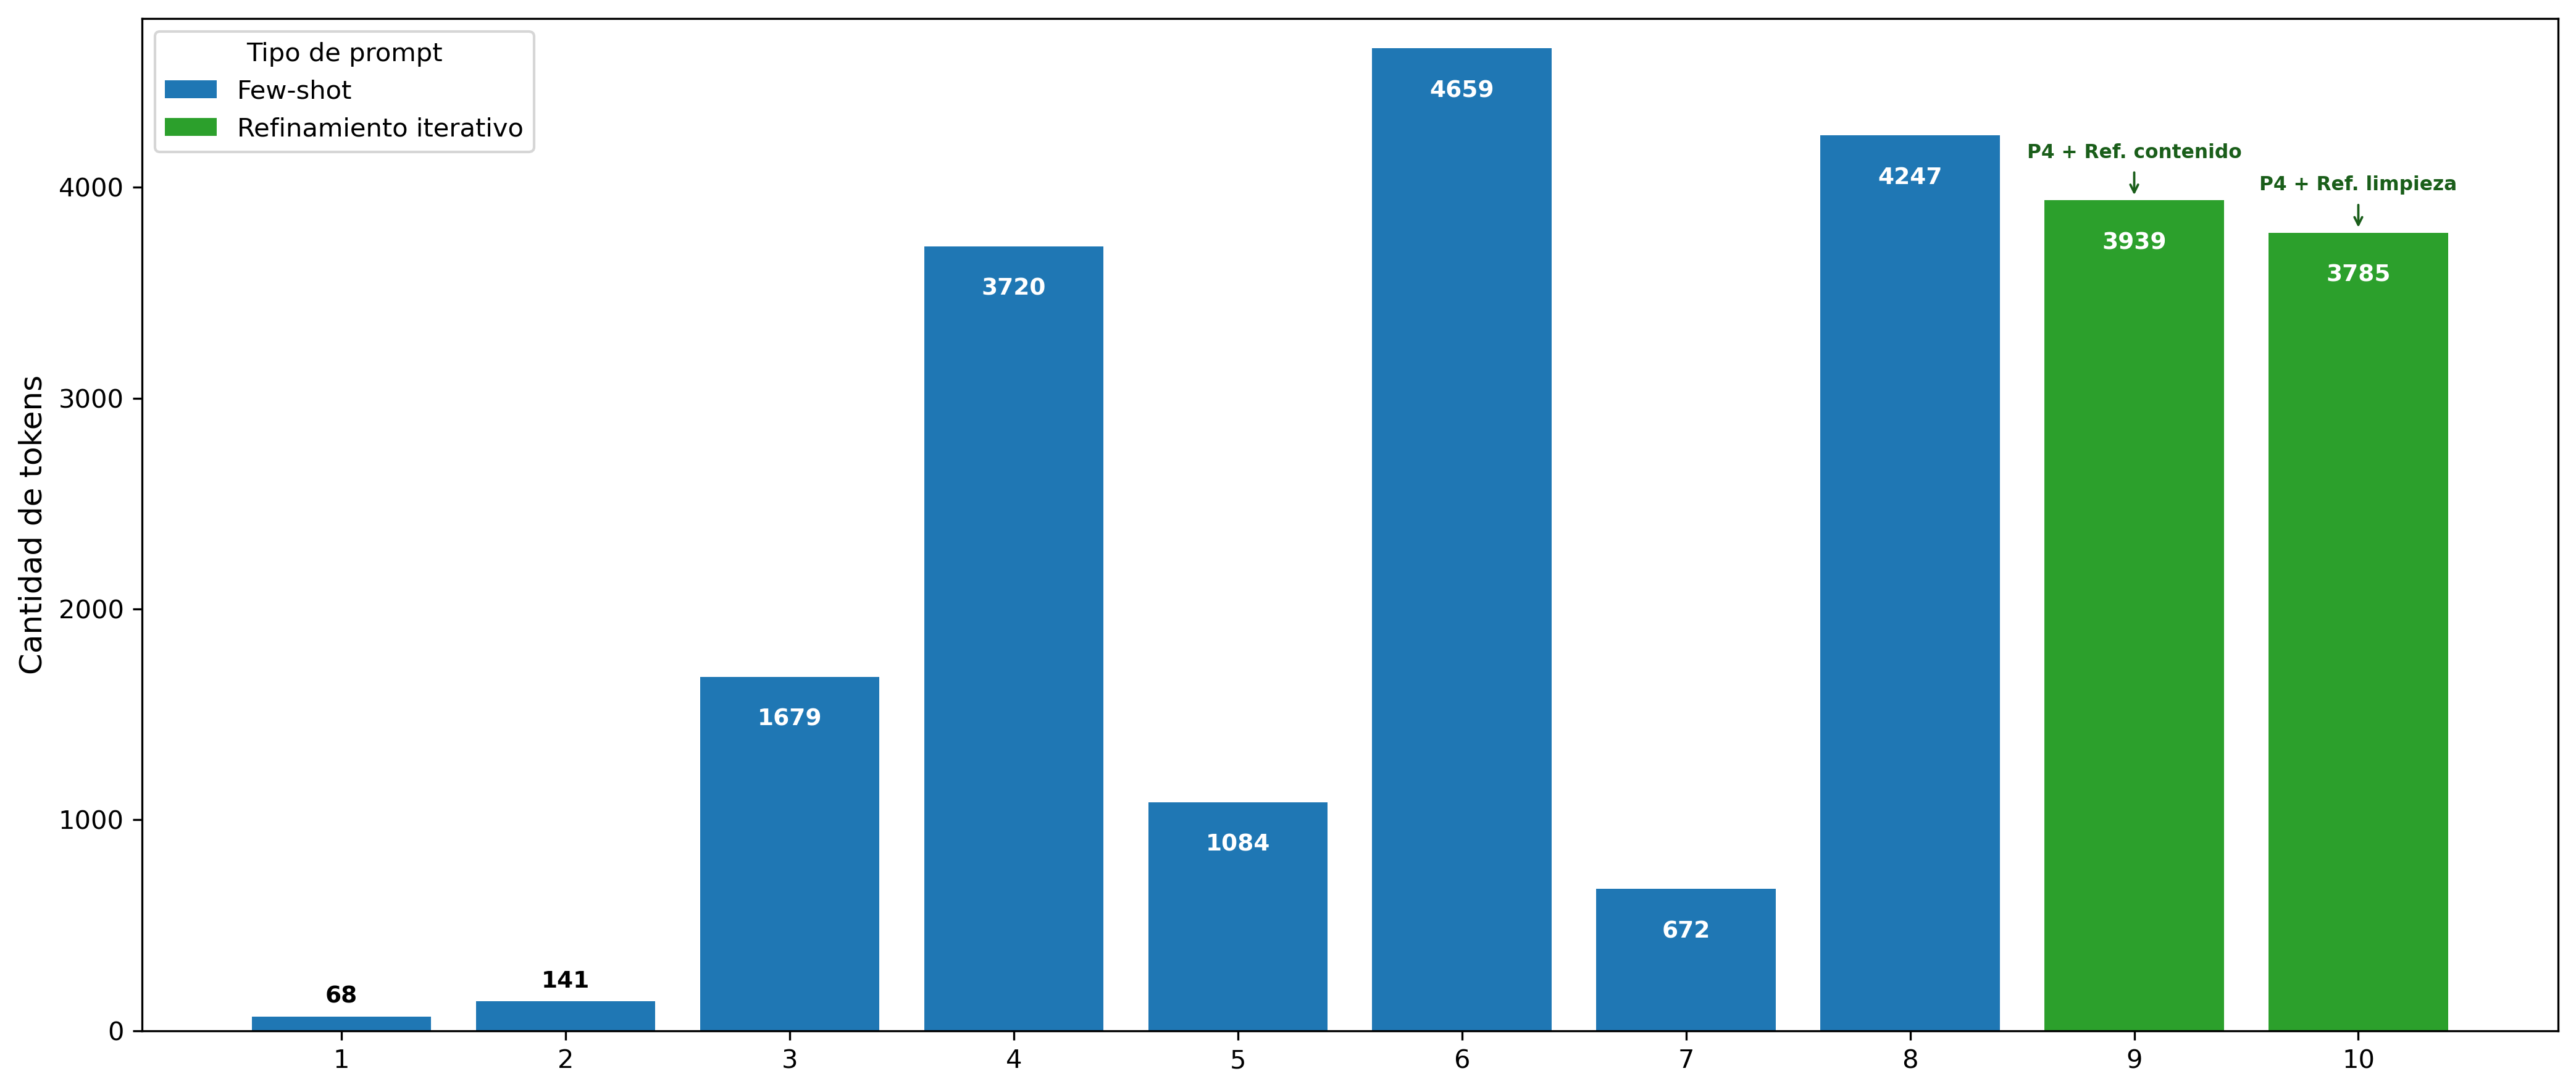
\includegraphics[width=\textwidth]{Graficos_Tesis/grafico_tokens_adaptacion.png}
  \caption{Cantidad de tokens por prompt, promediada entre las versiones diseñadas para los niveles A2 y B1. Las barras azules corresponden a prompts directos con información lingüística explícita few-shot. Las barras verdes (experimentos~9 y 10) representan procedimientos de refinamiento iterativo: se aplica primero el prompt~4 para obtener una adaptación inicial, seguido de un segundo prompt.}
  \label{fig:grafico_tokens_adaptacion}
\end{figure}


\subsubsection{Recursos lingüísticos utilizados}
Un aspecto distintivo de los experimentos de adaptación respecto a los de clasificación es el uso de recursos lingüísticos especializados incorporados directamente en los prompts. Estos recursos incluyen vocabulario graduado por nivel CEFR y ejemplos de construcciones morfosintácticas características de los niveles A2 y B1, que corresponden a los niveles objetivo de la tarea. Los recursos lingüísticos compilados para este trabajo se encuentran disponibles públicamente en este repositorio \cite{oviedo2024recursos} que recopila los datos utilizados a lo largo del trabajo.


\subsection{Tarea objetivo y marco de evaluación}
Los experimentos se enmarcan en la shared task TSAR 2025, que propone simplificar textos de nivel B2 o superior hacia niveles A2 o B1. Por lo tanto, a diferencia del capítulo de clasificación, donde se trabajó con los seis niveles del CEFR, aquí el foco se restringe a la dirección de simplificación: textos complejos como entrada y textos de menor complejidad como salida. Esta restricción es coherente con las necesidades pedagógicas identificadas en la motivación del trabajo, donde el caso más frecuente es el de un docente que necesita adaptar un material existente a un nivel inferior al de su formulación original.

De acuerdo con las bases de la competencia, se permitió el envío de hasta tres variantes o estrategias distintas (runs) para ser evaluadas formalmente. Para este trabajo, se seleccionaron tres aproximaciones con niveles crecientes de complejidad y esfuerzo de diseño, tras una evaluación sistemática sobre los datos de prueba y una inspección cualitativa de los textos generados, los prompts detallados para cada run se encuentran en [cite].

\subsubsection{Estrategias de Adaptación}

\noindent\textbf {Run 1: Refinamiento iterativo y preservación de contenido}

Esta estrategia aborda la tensión entre la adecuación al nivel objetivo y la fidelidad al mensaje original mediante un procedimiento de dos pasos:

\begin{enumerate}
\item \textbf{Adaptación Inicial (Prompt extenso):} Se utiliza un prompt de aproximadamente 3.800 tokens que incorpora descriptores de lectura de A2 y B1 {CouncilEurope2020} [cita], listas de vocabulario de {Oxford3000} [cita] (872 palabras para A2 y 809 para B1) y una lista de 5 ejemplos para cada nivel para cada tipo de construcciones morfosintácticas {North2010}[cita], un total de 190 oraciones, 105 para A2 y 85 para B1.
\item \textbf{Refinamiento de Contenido:} La salida anterior se procesa con un segundo prompt orientado exclusivamente a la preservación del contenido. Esta etapa prioriza la fidelidad semántica sobre la adecuación lingüística, intentando mitigar la pérdida de información que suele ocurrir en prompts excesivamente largos.
\end{enumerate}

\noindent\textbf {Run 2: Refinamiento iterativo y corrección de meta-información}
Basada en la misma configuración inicial del Run 1, esta estrategia busca solucionar un problema recurrente observado en los modelos de lenguaje: la inclusión de meta-explicaciones (ej. ``Aquí tienes el texto simplificado...''). A pesar de las instrucciones negativas en el prompt original, el modelo tiende a justificar su tarea. Por ello, el segundo paso de esta estrategia consiste en un prompt de ``limpieza'' diseñado para detectar y eliminar cualquier fragmento de texto que no sea la adaptación propiamente dicha.

\noindent\textbf {Run 3: Sistema de votación}

Esta es la estrategia más compleja y la que obtuvo los mejores resultados. Consiste en generar diez adaptaciones distintas del mismo texto de entrada utilizando diez prompts de diversa naturaleza (desde instrucciones simples hasta few-shot). Las diez salidas son evaluadas por un mecanismo de votación heurístico basado en cuatro criterios:

\begin{itemize}
\item \textbf{Ausencia de meta-información:} Penalización de 10 puntos si el texto contiene secuencias explicativas de la tarea.
\item \textbf{Adecuación al nivel CEFR:} Se utilizan tres clasificadores proporcionados por la organización. Se penaliza la discrepancia entre el nivel predicho y el objetivo para cada clasificador, aumentando la penalidad según la distancia en la escala CEFR.
\item \textbf{Control de longitud:} Penalización de textos que superen en más de un 30\% la longitud del original, ya que las adaptaciones extensas suelen incluir alucinaciones o información redundante.
\item \textbf{Similitud semántica:} Evaluación mediante MeaningBERT [cita]. Si la similitud con el original es menor a 0.6, se aplica una penalización de 5 puntos, esto fue realizado en base a un criterio empirico con el objetivo de preservar al menos dos tercios del significado.
\end{itemize}

En caso de empate en la puntuación, se selecciona el texto con mayor similitud semántica o, en última instancia, aquel generado por el prompt con mejor desempeño histórico en los datos de prueba.

\subsection{Métricas de Evaluación}

Para evaluar el desempeño de los sistemas de adaptación, se describe el marco de evaluación propuesto por la shared task TSAR 2025, el cual se basa en el estándar AUTORANK {Kocmi2025} [cita], para luego dar los resultados obtenidos en la tarea. Este enfoque combina múltiples métricas en un ranking único, permitiendo evaluar tres dimensiones críticas: el cumplimiento del nivel CEFR, la preservación del significado y la similitud con las referencias de expertos.

\subsubsection{Dimensiones de Medición}

Se utilizaron tres variables principales para cuantificar la calidad de las adaptaciones generadas:

\begin{itemize}
    \item \textbf{Cumplimiento del nivel CEFR:} Se utiliza el Error Cuadrático Medio (RMSE) calculado a partir de un modelo evaluador CEFR entrenado específicamente para la tarea. A diferencia de la precisión simple, el RMSE penaliza las predicciones de forma proporcional a su distancia respecto al nivel objetivo (por ejemplo, clasificar un texto como B2 cuando el objetivo es A2 recibe una penalización mayor que si se clasificara como B1).

    \item \textbf{Preservación del Significado:} Se emplea MeaningBERT para medir la similitud semántica entre el texto original y la salida del sistema. MeaningBERT es preferible a métricas generales como BERTScore, ya que ha sido entrenado específicamente con anotaciones humanas sobre preservación de significado en tareas de simplificación.
    
    \item \textbf{Similitud con Referencias:} Se utiliza nuevamente MeaningBERT para comparar la salida del sistema con las simplificaciones escritas por expertos (gold-standard). Esta métrica es crucial, ya que la similitud con una referencia humana suele correlacionar mejor con la calidad pedagógica de la adaptación.
\end{itemize}

\subsubsection{Normalización y Ponderación}

Dado que las métricas operan en escalas distintas (el RMSE puede tener varianzas altas mientras que MeaningBERT presenta valores agrupados), se aplica una normalización basada en el escalado de mediana e interpercentil (median-interpercentile scaling). Este método reduce la influencia de valores atípicos y permite que las métricas sean comparables entre sí. En el caso del RMSE, los valores se invierten tras la normalización para que, en todos los indicadores, una puntuación más alta represente un mejor desempeño.

Para obtener el puntaje final de cada run, se asignan pesos específicos que equilibran el control de legibilidad y la fidelidad semántica:
\begin{itemize}
    \item \textbf{Cumplimiento del nivel CEFR:} 50\% (peso de 0.500).
    \item \textbf{Preservación del Significado:} 16.7\% (peso de 0.167).
    \item \textbf{Similitud con Referencias:} 33.3\% (peso de 0.333).
\end{itemize}

La decisión de otorgar el doble de peso a la similitud con la referencia respecto a la similitud con la fuente responde a que la primera refleja con mayor precisión el criterio de expertos sobre lo que constituye una simplificación exitosa.

%\subsubsection{Agregación y Ranking Final (AUTORANK)}

%Tras la normalización y ponderación, se calcula un promedio ponderado para cada sistema. Estos puntajes se mapean linealmente en un rango de $[1, N]$, donde $N$ es el número total de envíos válidos. Bajo la convención de AUTORANK, el sistema con mejor desempeño recibe el valor 1, mientras que el de menor rendimiento recibe el valor $N$. Este mecanismo permite una interpretación clara de la posición relativa de cada estrategia frente al estado del arte actual en la competencia.

\subsection{Resultados y Discusión}\label{sec:ad_resultados}

En este apartado se presentan y analizan los resultados obtenidos por las tres estrategias de adaptación (runs) enviadas a la shared task TSAR 2025. Los resultados se evalúan siguiendo el marco oficial de la competencia, destacando el desempeño de nuestro sistema,\textit{TaskGen}, en comparación con el estado del arte.

\subsubsection{Análisis comparativo de los sistemas enviados}

De acuerdo con el reporte oficial de la competencia {alva-manchego-etal-2025-findings} [cita], nuestra tercera estrategia (\textbf{Run 3}), basada en un \textit{ensemble} por votación, obtuvo el mejor desempeño entre los envíos de nuestro equipo. Esta estrategia se posicionó como la 13ª mejor entre todos los participantes, situando a \textit{TaskGen} en el 6º lugar del ranking general por equipos. Aunque el RMSE respecto al nivel CEFR fue aceptable, con un promedio de 0,628, esta ejecución destacó en la preservación del significado respecto al original (meaning-orig) y a la referencia ( meaning-ref), con valores de 0,856 y 0,826 respectivamente.

En la \Cref{tab:results_metrics_tsar} se resumen las métricas principales para los tres sistemas.

\begin{table}[H]
    \centering \small
    {\renewcommand{\arraystretch}{1.2}
    \begin{tabular}{l|ccccc}
     & {\bf RMSE} & {\bf meaning-orig} & {\bf meaning-ref} \\\hline%& AvgScore & AUTORANK
    {\bf Run1} & 0.592 & 0.791 & 0.786 \\%& -0.084 & 10.070  
    {\bf Run2}& 0.561 & 0.752 & 0.773 \\%& -0.169 & 11.150 \\\hline
    {\bf Run3} & {\it 0.628} &  {\it 0.856} & {\it 0.826} \\%& 0.122 & 7.480 \\\hline
    \end{tabular}}
    \caption{Resultados de {\it TaskGen} en la shared task TSAR 2025.}
    \label{tab:results_metrics_tsar}
\end{table}

El análisis de los datos permite extraer las siguientes observaciones:

\begin{itemize}
    \item \textbf{Run 1 (Refinamiento de contenido):} Esta estrategia, que combinaba un prompt lingüístico extenso con un segundo paso de adecuación de contenido, obtuvo un equilibrio aceptable, logrando un RMSE de 0.592. Sin embargo, su capacidad de preservación semántica fue inferior a la del \textit{ensemble}. En comparación con otras aproximaciones, obtuvo puntuaciones más bajas en la preservación del significado del texto original y en la similitud con la referencia (0,791 y 0,786 respectivamente), lo que situó a esta ejecución en la mitad inferior de los sistemas participantes.
    
    \item \textbf{Run 2 (Limpieza de meta-información):} Sorprendentemente, esta estrategia obtuvo el mejor desempeño en cuanto a adecuación al nivel CEFR objetivo (RMSE 0.561), aunque registró puntuaciones de preservación de significado más bajas que las del Run 1. Esto sugiere que el prompt de segundo paso utilizado en el Run 1 para la fidelidad semántica pudo haber interferido negativamente en el control de la legibilidad, mientras que la eliminación de meta-información permitió una salida más alineada con los descriptores del nivel.
    
    \item \textbf{Run 3 (Votación):} Aunque registró el peor RMSE de los tres (0.628), su desempeño en preservación de significado fue significativamente superior (0.856 respecto al original y 0.826 respecto a la referencia). Fue precisamente esta alta fidelidad semántica la que permitió que esta estrategia alcanzara el mejor ranking global bajo el marco AUTORANK.
\end{itemize}

\subsubsection{Análisis por nivel objetivo: A2 vs. B1}

Dado que el cumplimiento del nivel CEFR fue el punto donde se observó mayor variabilidad, realizamos un análisis mas detallado por nivel objetivo. Como se observa en las \Cref{fig:rmse,fig:clasificacion_cuadrantes_global} las estrategias de refinamiento y limpieza,  mostraron mayores dificultades para adaptar textos hacia el nivel B1, mientras que el éxito fue al adaptar hacia el nivel A2, por otro lado la estrategia de votación, el desempeño fue mejoro un poco sobre B1, pero bajo mucho su rendimiento en A2. Esto puede deberse a que el sistema de votacion penaliza mas fuertemente la fidelidad semantica, quedando en menores posiciones las adaptaciones que logran un mejor cumplimiento del nivel CEFR pero a costa de una mayor perdida de significado, lo que se refleja en el RMSE mas alto con respecto a los otros runs y especialmente hacia A2.

Una observacion sobre el RMSE, es que como se vio en la seccion de clasificacion [cita], el clasificador utilizado para evaluar el cumplimiento del nivel CEFR no es capaz de clasificar textos como A1, lo que implica que cualquier texto adaptado a A2 que presente una complejidad cercana a A1 será clasificado como A2, lo que podría explicar la aparente mejor adecuación al nivel A2 en comparación con B1, donde el margen de error es mayor.

No obstante, los errores detectados fueron menores: la mayoría de los casos corresponden a una discrepancia de un solo nivel, textos destinados a B1 que fueron clasificados como A2. Estos casos serán analizados en profundidad en etapas posteriores para mejorar la precisión del sistema.

Por otro lado, la preservación del significado mostró un comportamiento inverso, como ilustra la estimación de densidad de la \Cref{fig:density,fig:clasificacion_cuadrantes_global}. La fidelidad semántica fue notablemente superior en las adaptaciones hacia B1 que hacia A2 para todas las estrategias. Esto indica que a medida que el nivel objetivo desciende (mayor simplificación), la dificultad para preservar la totalidad del contenido original aumenta significativamente.

\begin{figure}[H]
  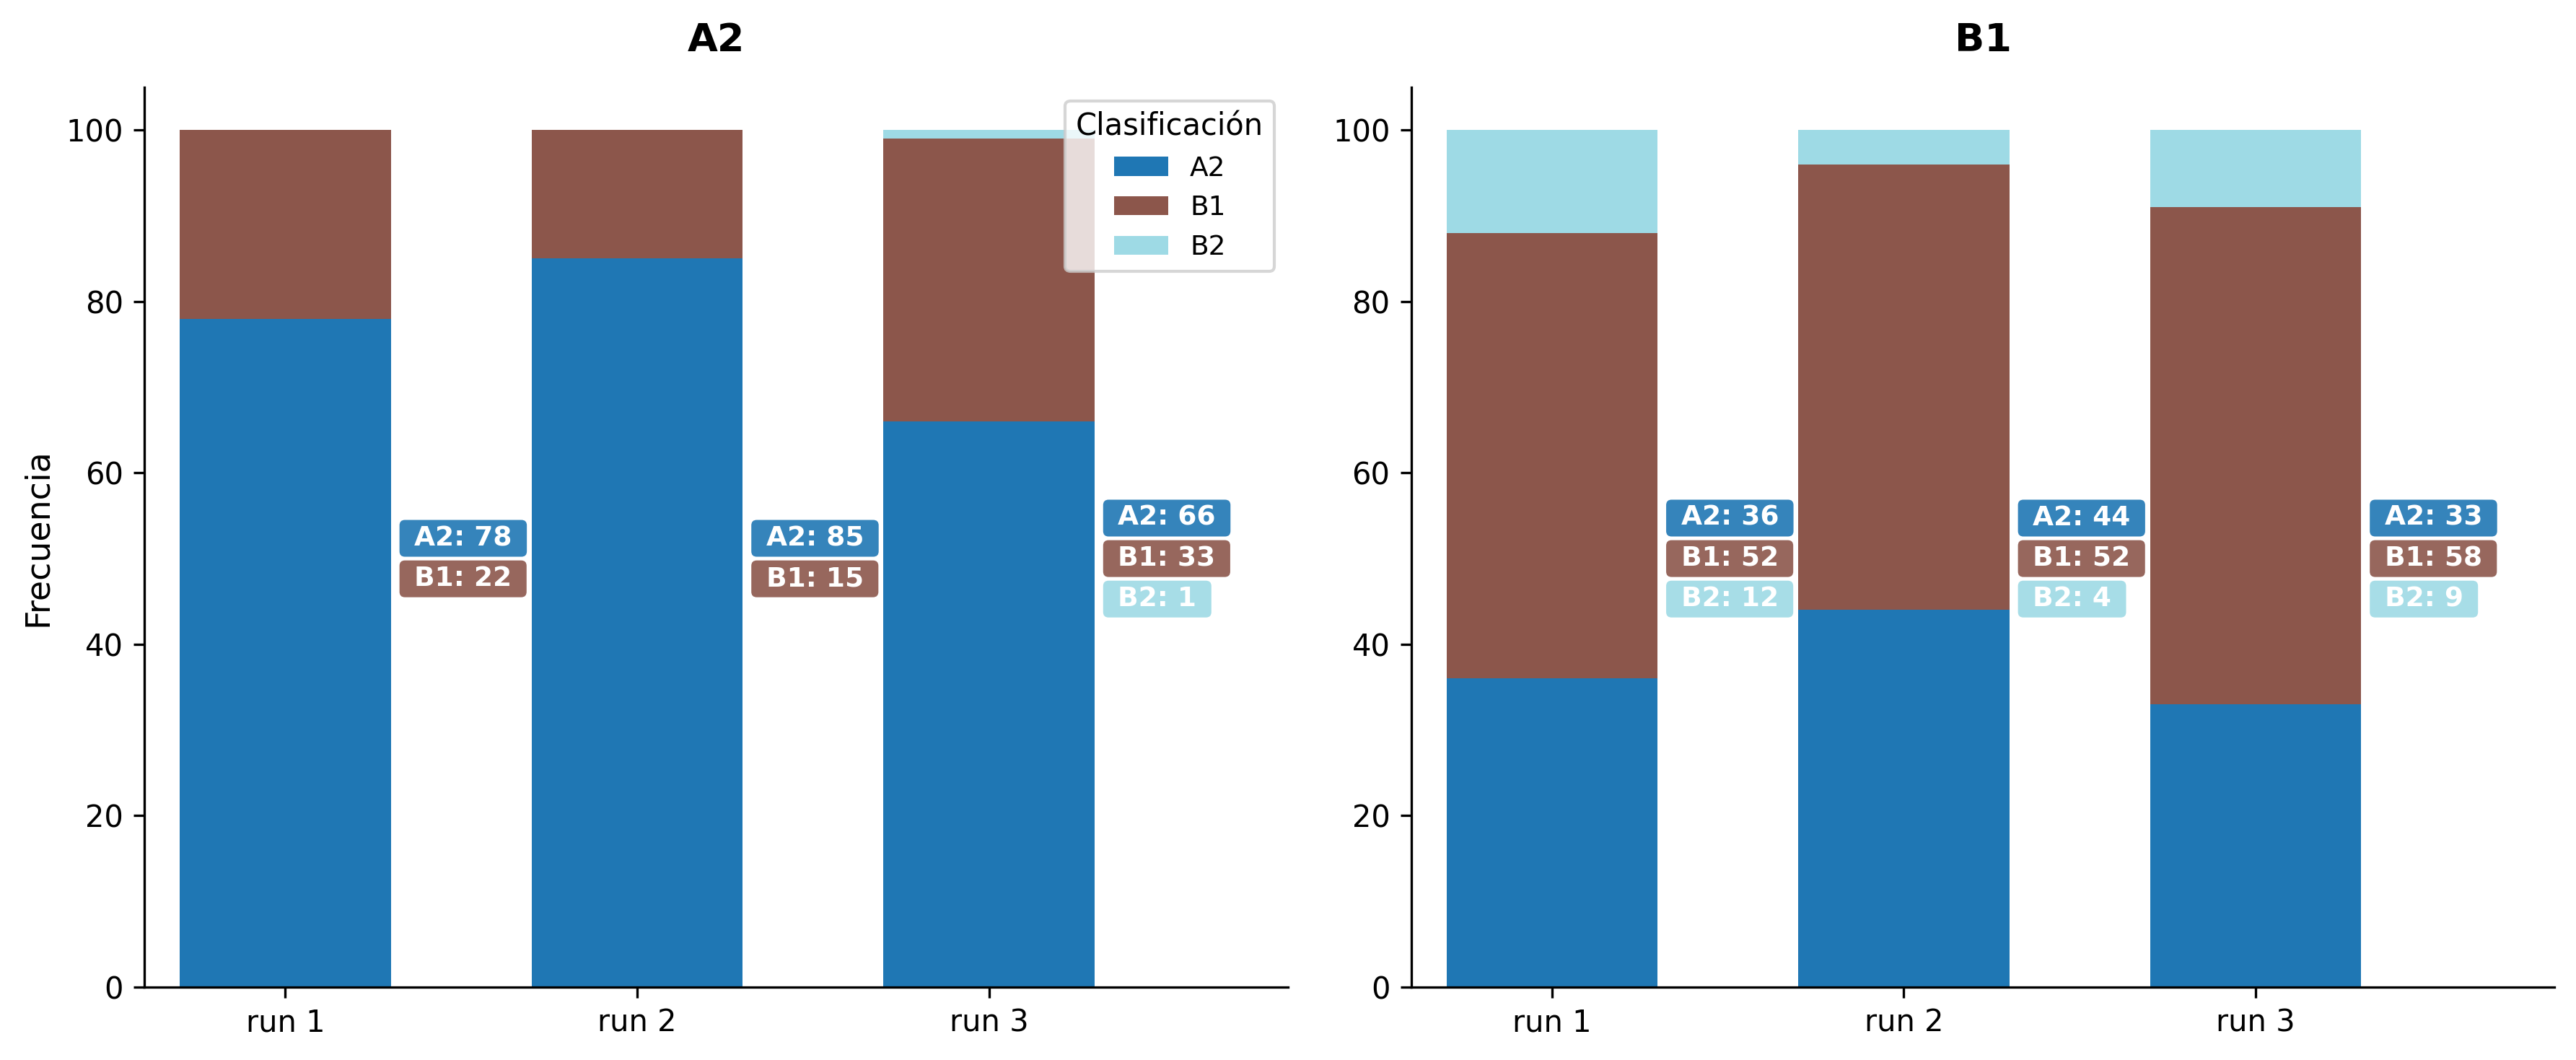
\includegraphics[width=\linewidth]{Graficos_Tesis/distancia.png} 
  \caption{Distribución de los niveles CEFR asignados por el clasificador a los textos adaptados para los niveles objetivo A2 (izquierda) y B1 (derecha). Cada barra representa una ejecución de una estrategia distinta}
  \label{fig:rmse}
\end{figure}

\begin{figure}[H]
  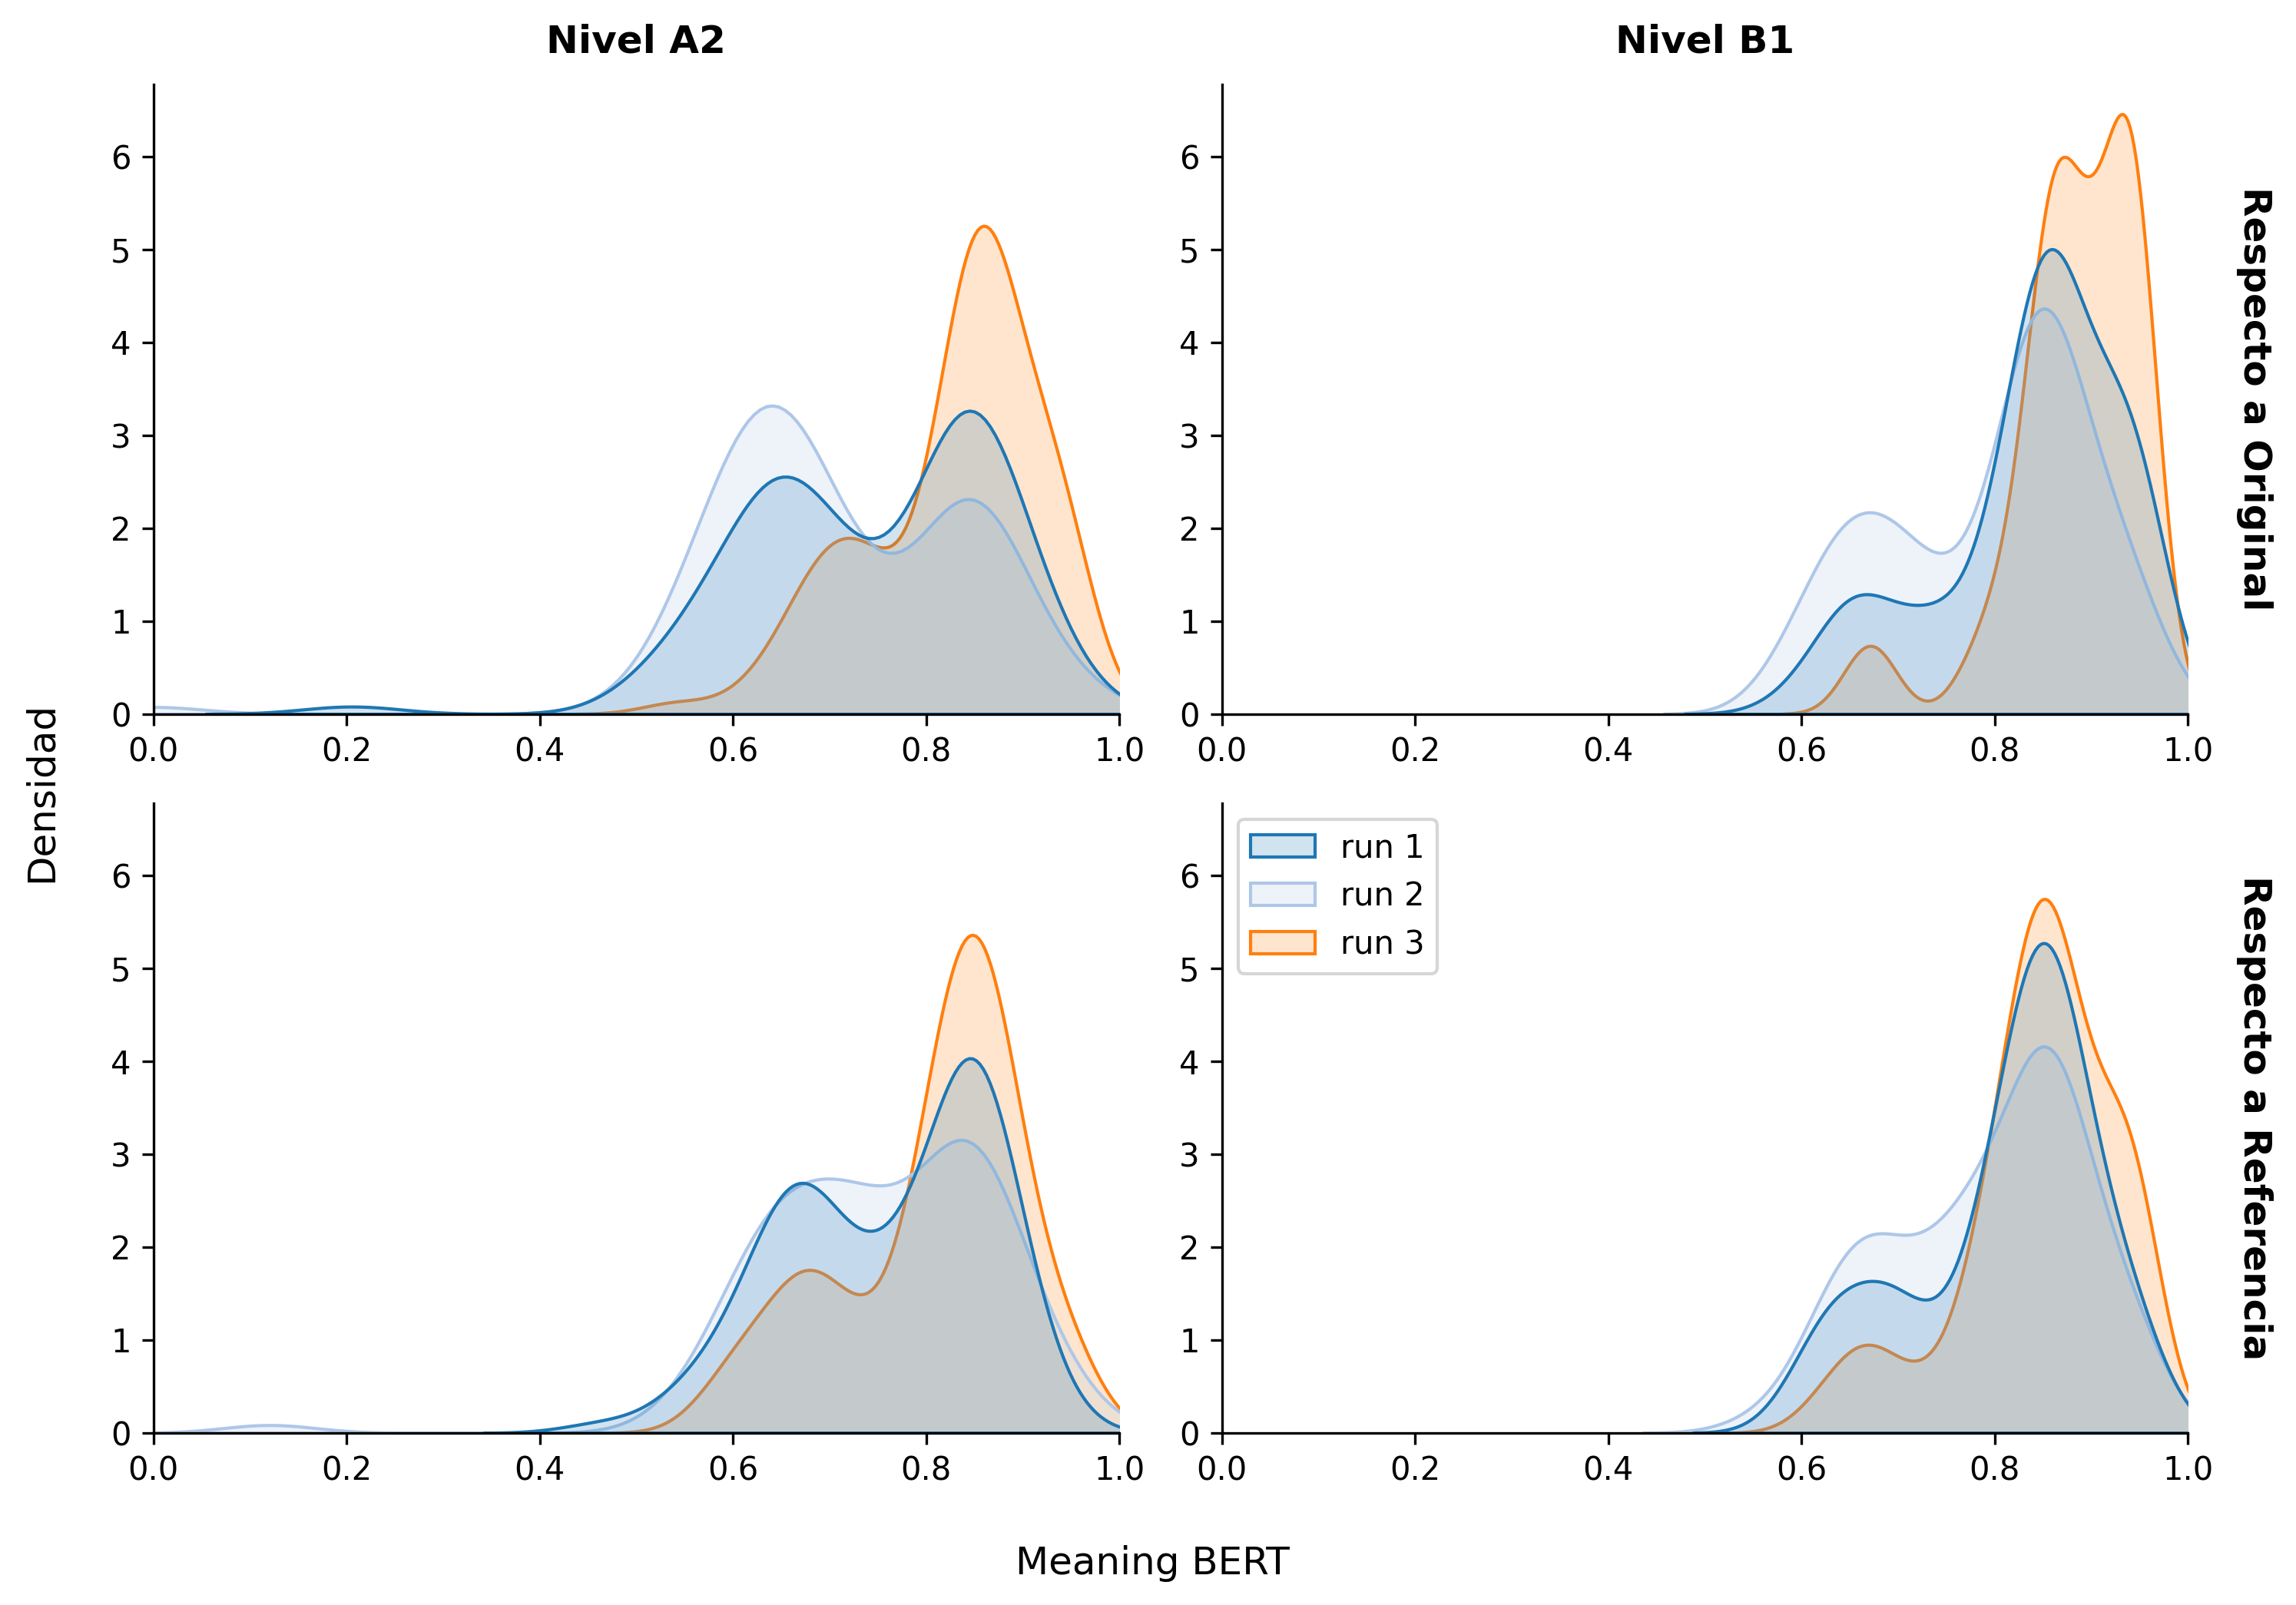
\includegraphics[width=\linewidth]{Graficos_Tesis/density_meaningbert_2x2_custom.png} 
  \caption {Estimación de densidad del puntaje de preservación de significado (MeaningBERT) respecto al original (arriba), respecto a la referencia (abajo), por nivel (A2 izquierda, B1 derecha).}
  \label{fig:density}
\end{figure}

\begin{figure}[H]
  \centering
  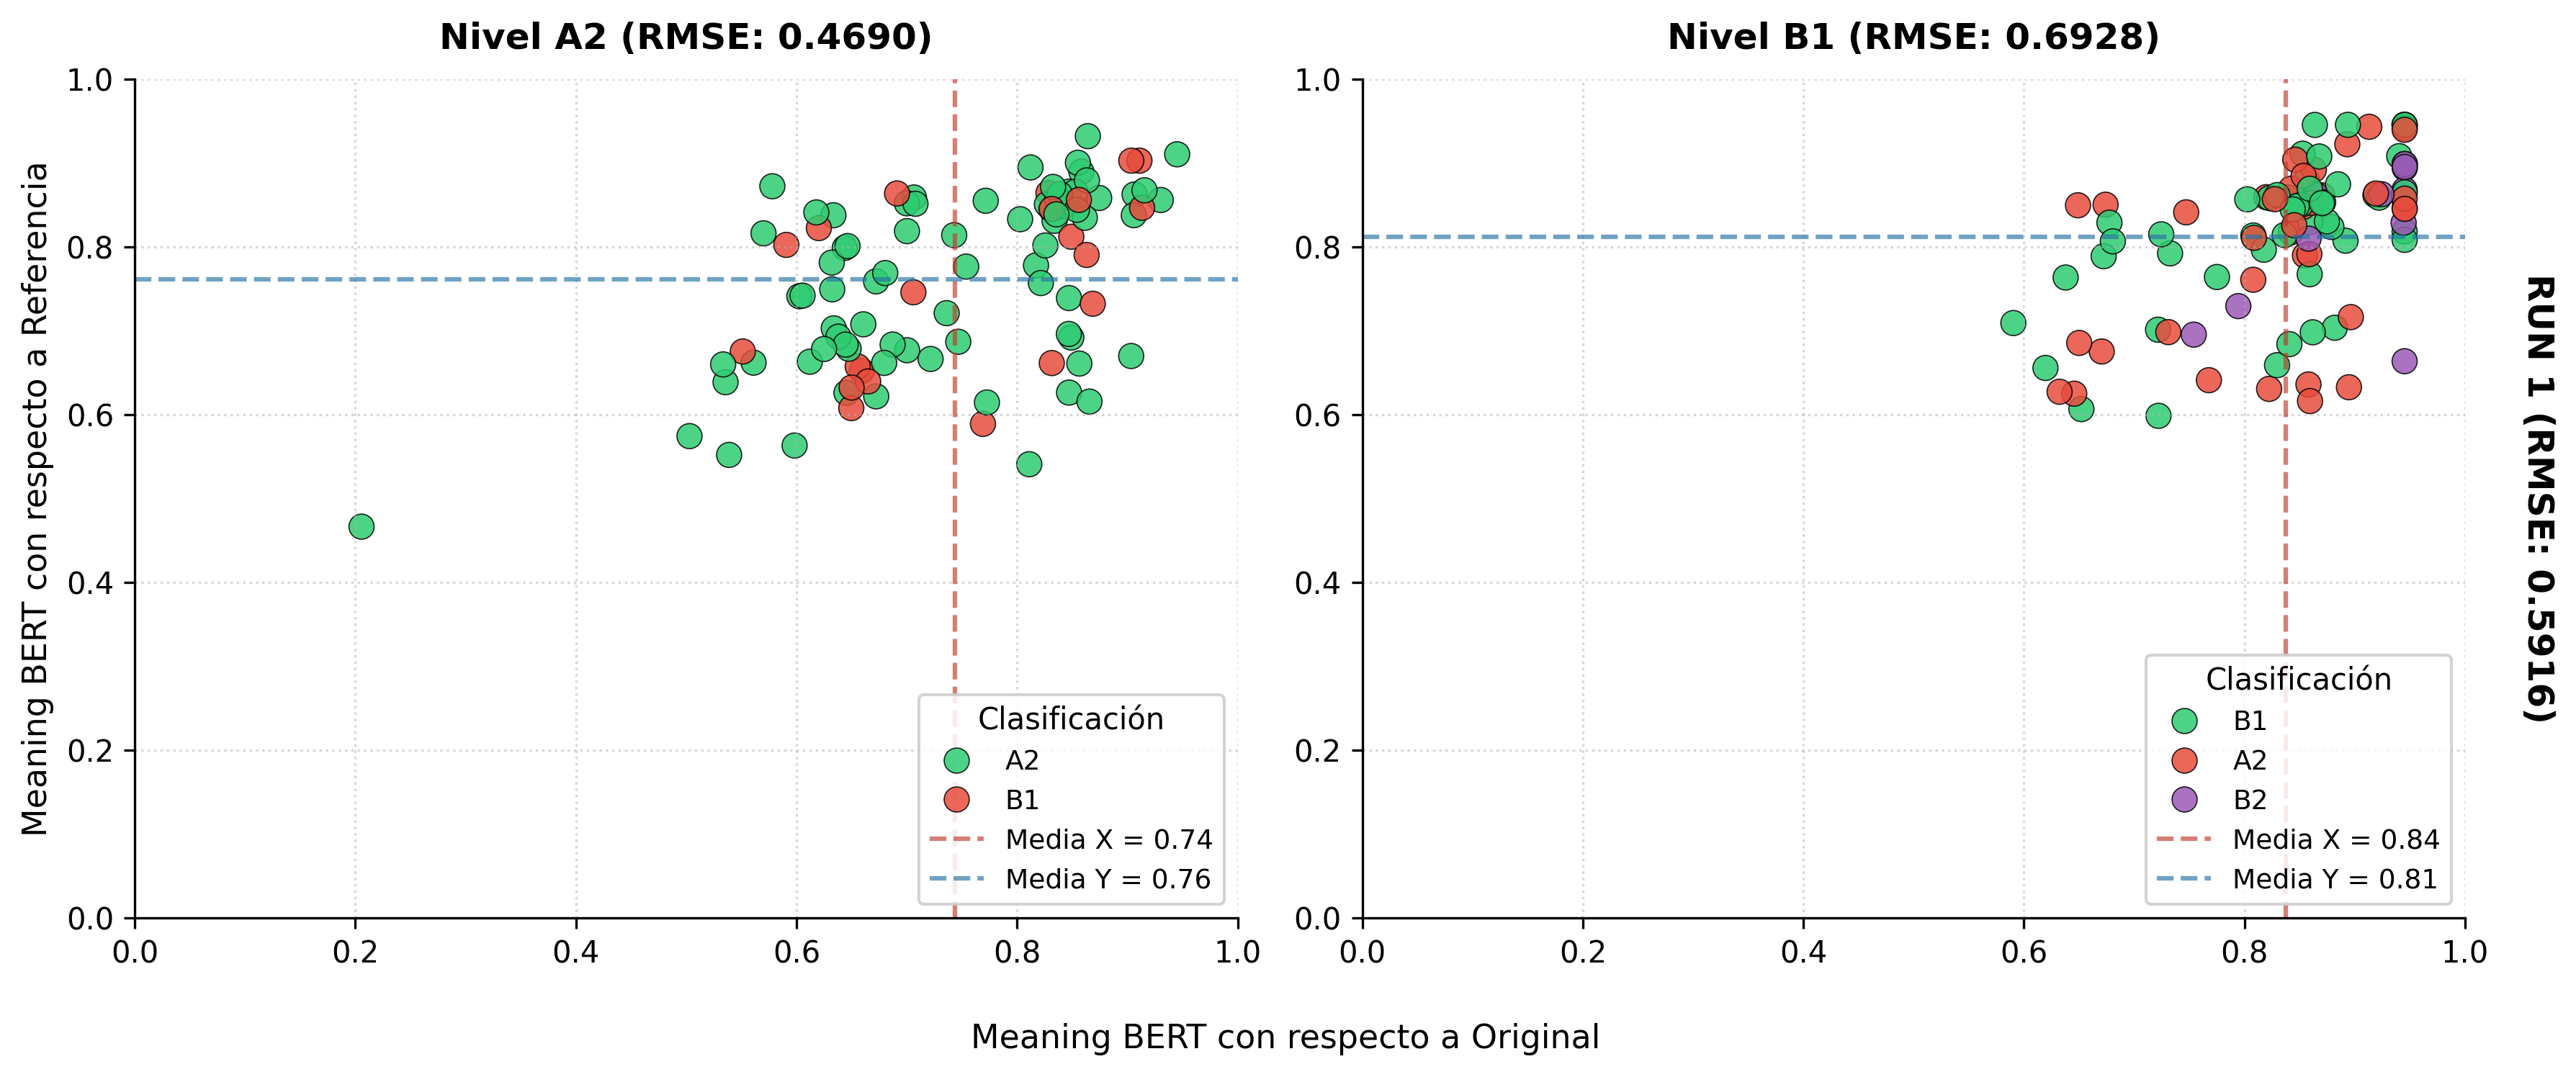
\includegraphics[width=\linewidth]{Graficos_Tesis/quadrant_classif_run_1.png}
  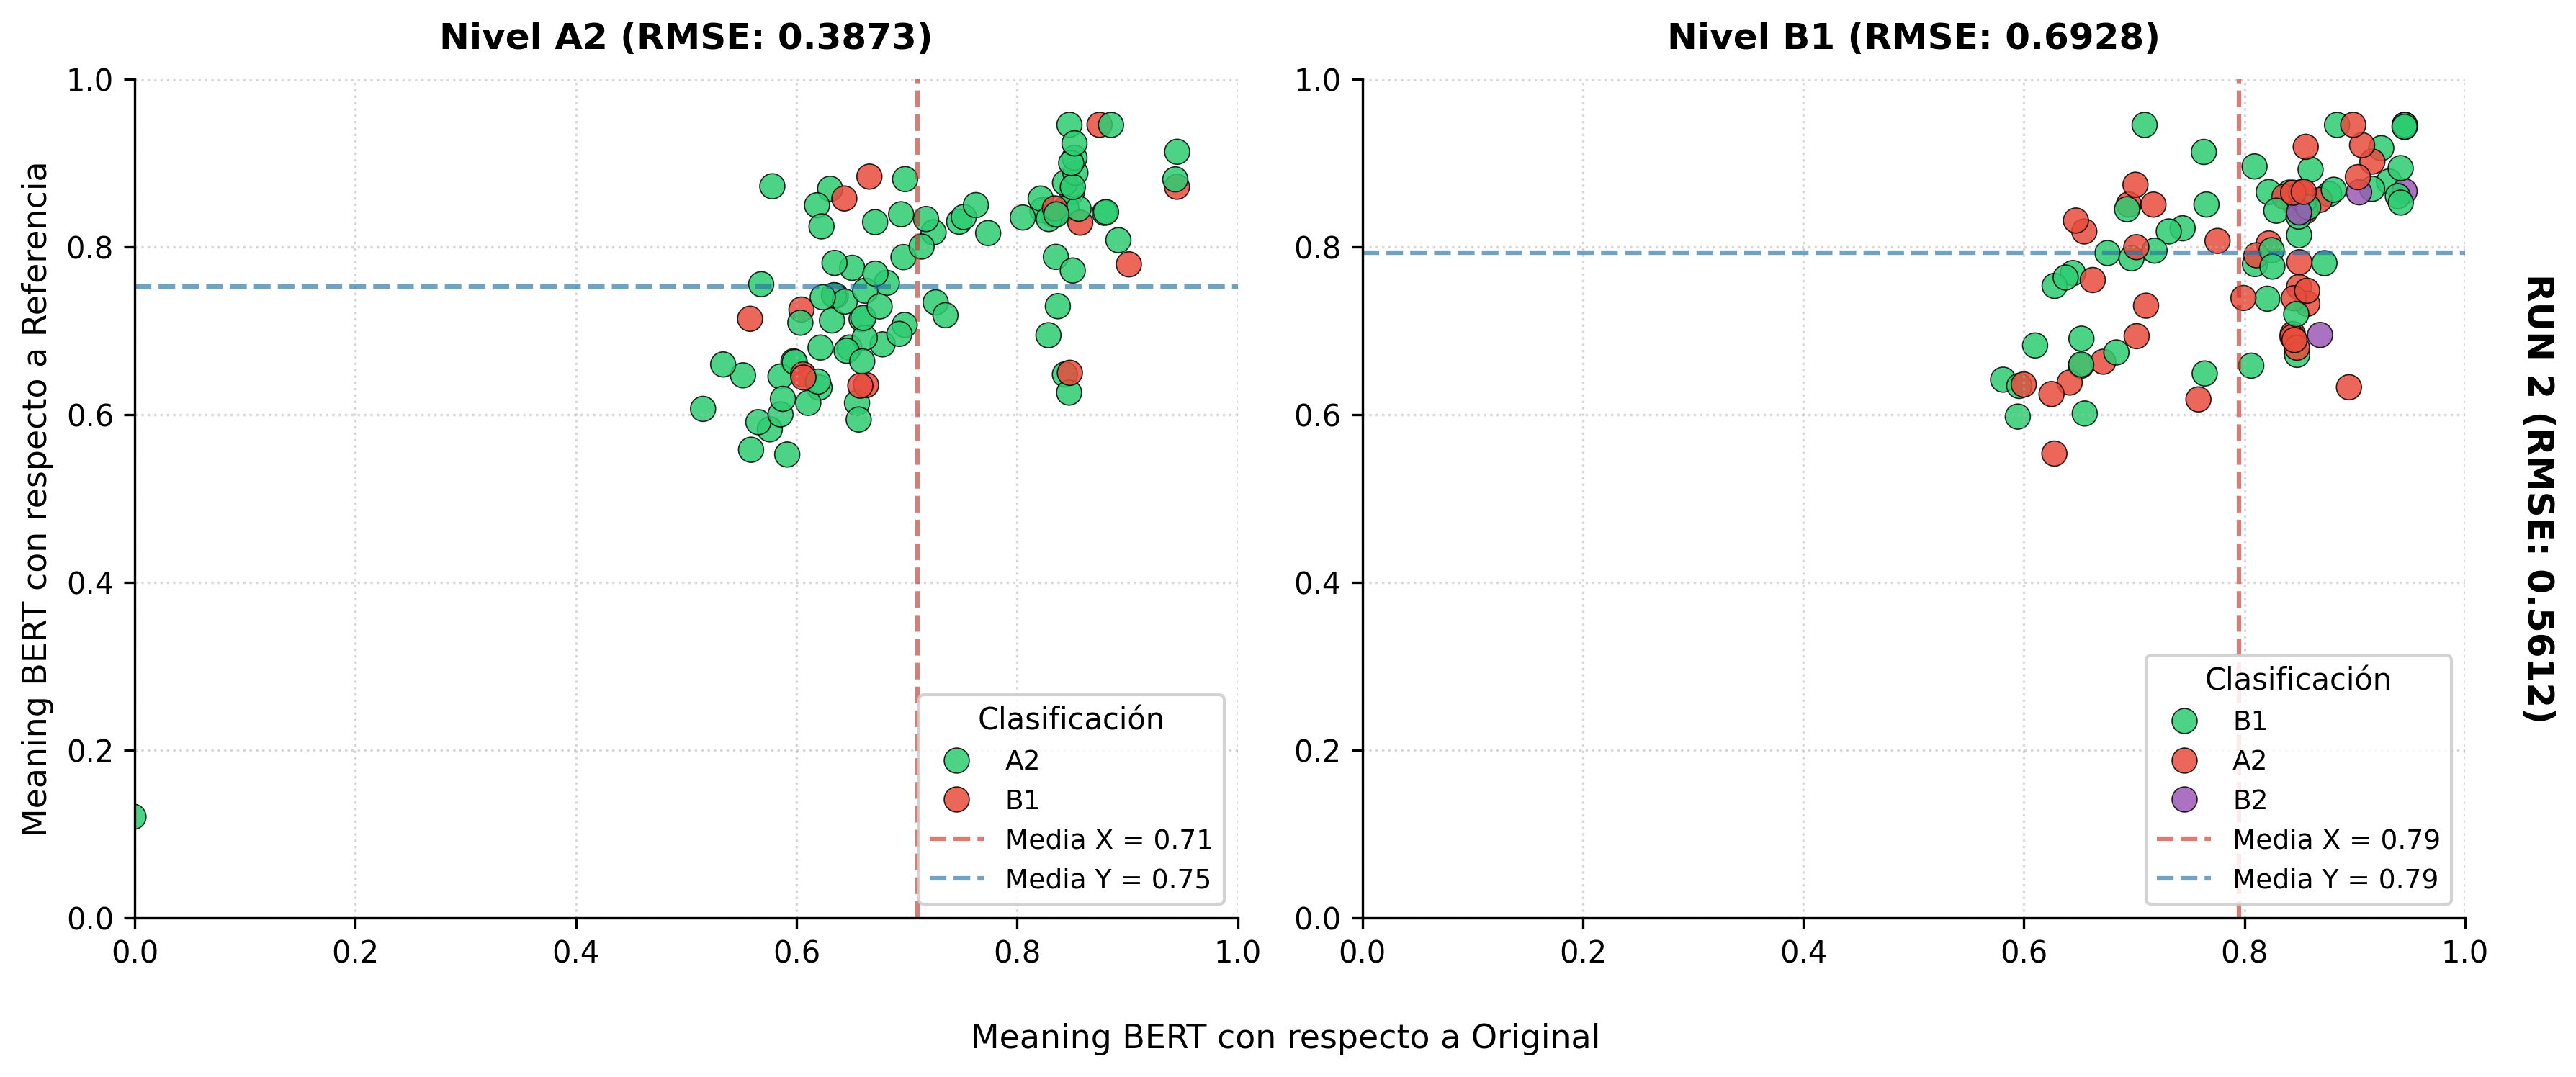
\includegraphics[width=\linewidth]{Graficos_Tesis/quadrant_classif_run_2.png}
  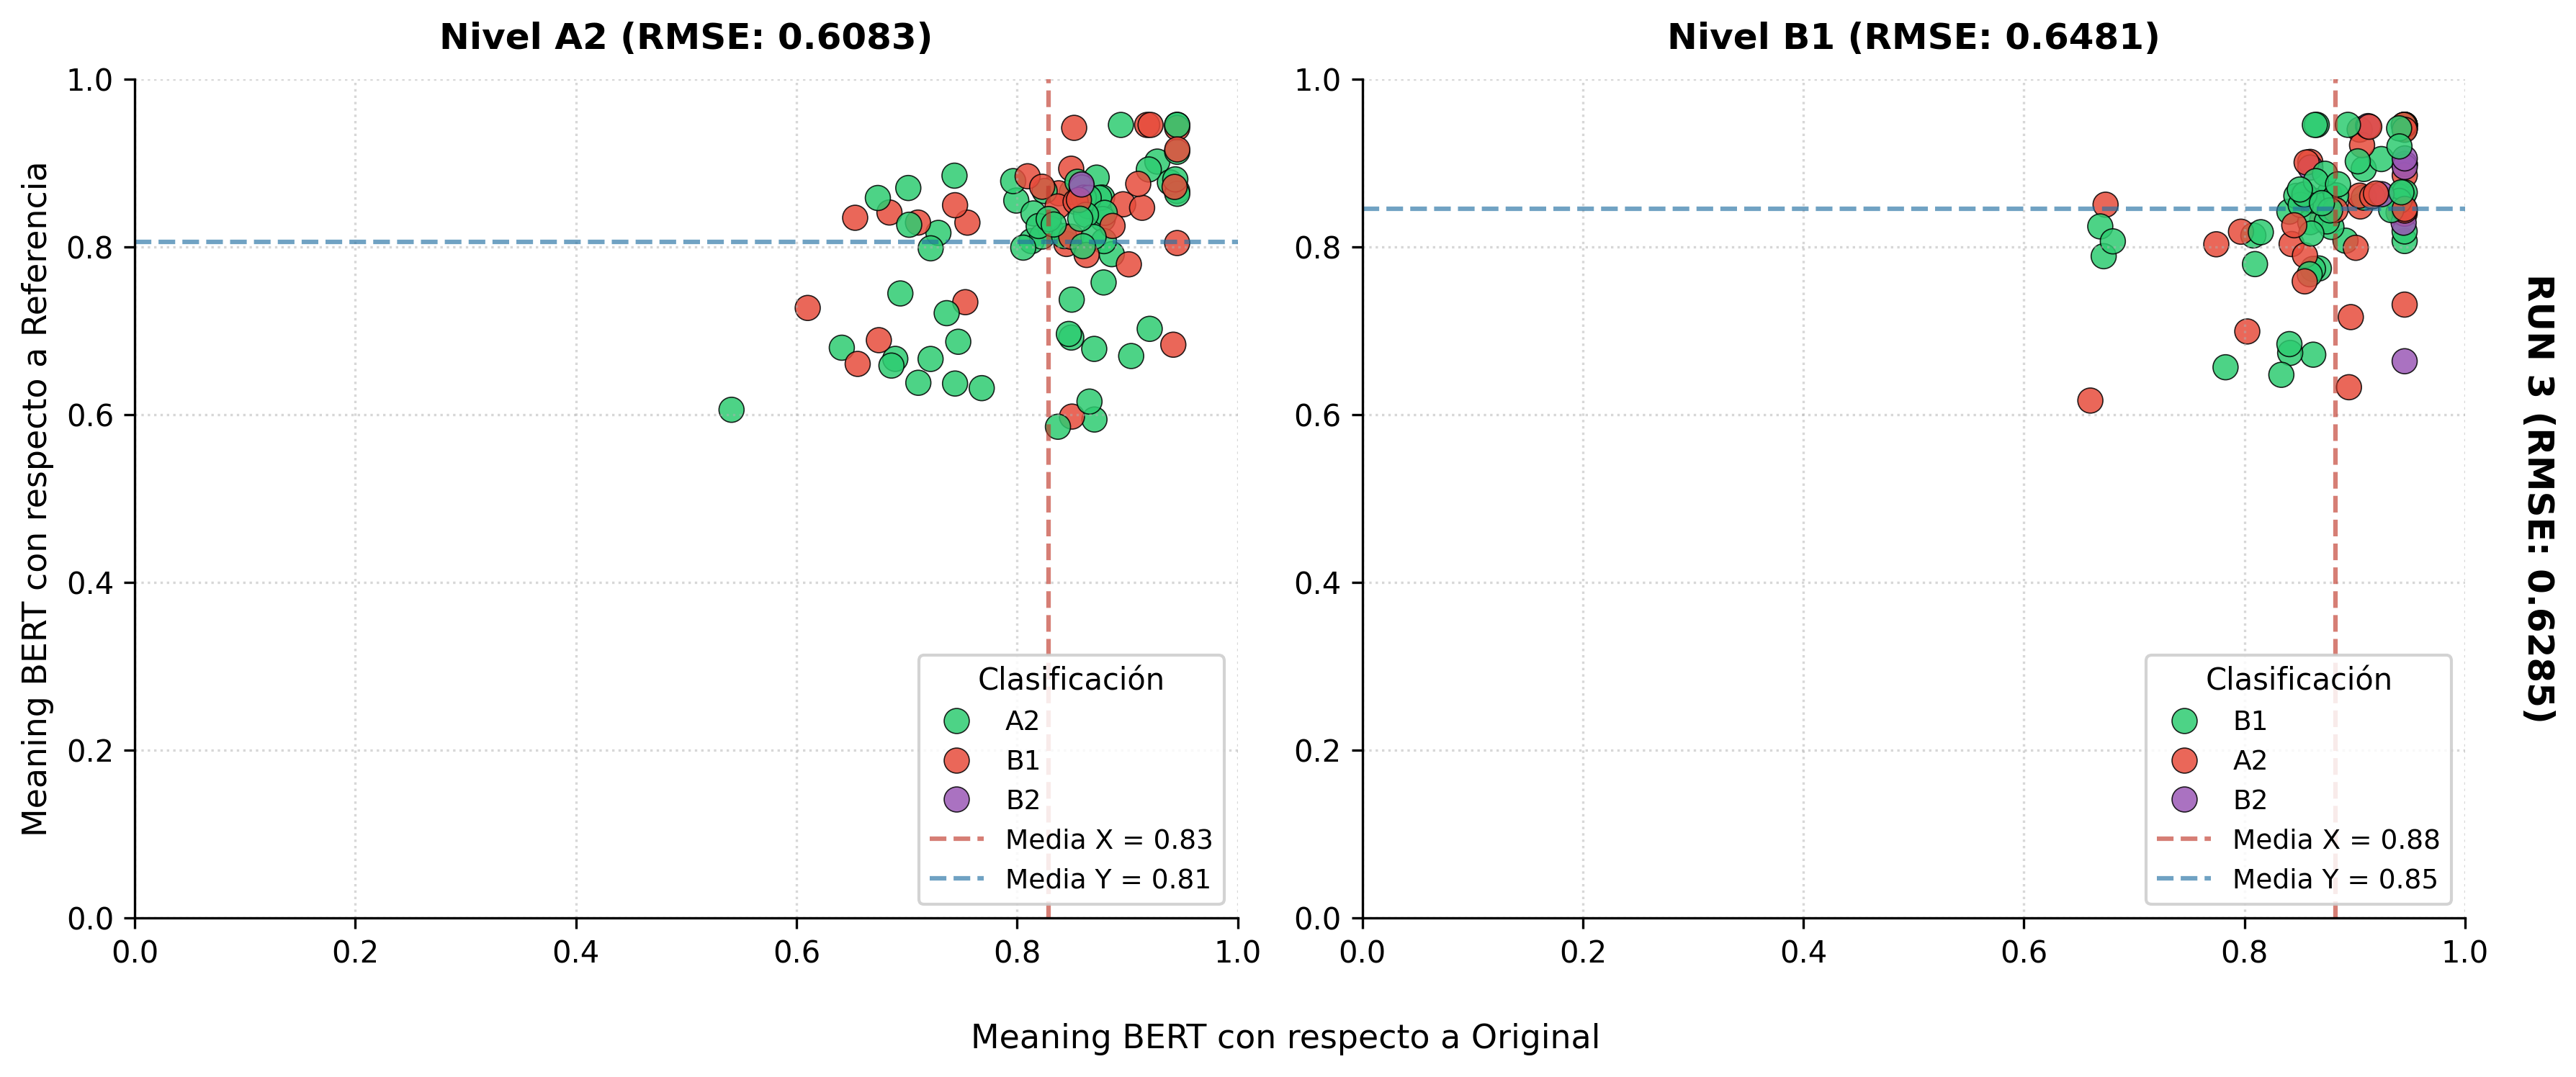
\includegraphics[width=\linewidth]{Graficos_Tesis/quadrant_classif_run_3.png}
  \caption{Análisis integral mediante gráficos de cuadrantes para las estrategias Run 1, 2 y 3 (arriba, medio, abajo). Cada gráfico contrasta la preservación semántica mediante MeaningBERT respecto al texto original (eje X) y a la referencia (eje Y), segmentado por nivel objetivo: A2 y B1 (izquierda, derecha). El color de los puntos individuales denota la clasificación CEFR obtenida. Se integran los valores de RMSE específicos por nivel objetivo (título superior) y el RMSE global de cada estrategia (margen derecho).}
  \label{fig:clasificacion_cuadrantes_global}
\end{figure}

\subsubsection{Ejemplos de salidas según los diferentes prompts}

Se observó que el Run 3 fue especialmente capaz de adaptarse a diferentes tipologías textuales. Por ejemplo, las \Cref{fig:orginal,fig:texto-run1,fig:texto-run2,fig:texto-run3} muestran cómo los Run 1 y 2 no lograron producir un resultado adecuado para un texto que resultaba particularmente desafiante, debido a que el modelo de lenguaje podía interpretarlo fácilmente como una instrucción en sí misma. No obstante, el Run 3 generó una mejor adaptación que los demás, aunque todavía existe margen de mejora.

Consideramos que es precisamente esta flexibilidad de la estrategia de ensemble para ajustarse a diversas tipologías de texto lo que la convirtió en nuestra mejor propuesta, alcanzando el 13º puesto entre todas las ejecuciones y posicionando a \textit{TaskGen} como el 6º mejor equipo en la competencia.

\begin{textexample}{}{Texto original}{fig:orginal}
Don't always follow positive feedback with negative feedback. When positive and negative feedback always appear to go hand in hand, the positives can become devalued and ignored. Ensure there are times when positive feedback is given for its own sake and resist the temptation to offer constructive criticism.
\end{textexample}


\begin{textexample}{}{Resultado de la estrategia 1 para nivel A2}{fig:texto-run1}
You give good feedback. You say nice things to your students.
\end{textexample}

\begin{textexample}{}{Resultado de la estrategia 2 para nivel A2}{fig:texto-run2}
You are a good teacher. You are kind to your students. Your students like you.
\end{textexample}

\begin{textexample}{}{Resultado de la estrategia 3 para nivel A2}{fig:texto-run3}
Don't always say something is wrong. When we say something is wrong and then something is right, people start to ignore the good things. We should say something is good just because it is good.
For example, a student does a good job on a test. We should just say, ``Well done!'' and not add ``But you could have done it faster.'' Or a friend helps us with something. We should say, ``Thank you!'' and not say ``You could have done it better next time.''\newline
This way, people will appreciate the good things and feel happy when we give them positive feedback.
\end{textexample}


\subsubsection{Impacto de las estrategias complejas}
Para evaluar el valor añadido de las estrategias de múltiples pasos, comparamos el desempeño de los prompts individuales frente a las ejecuciones combinadas (\Cref{tab:results_metrics_tsar_all}) sobre los datos de evaluacion. En particular, el prompt 4 sirvió como el prompt base para los Run 1 y 2.

\begin{table}[H]
    \centering
    \resizebox{\linewidth}{!}{
    \begin{tabular}{llrrr} % Adjusted to 8 columns based on your data
    \hline
    \textbf{Exp.} & \textbf{Prompt} & \textbf{RMSE} & \textbf{Meaning-orig} & \textbf{Meaning-ref} \\ \hline
    \textbf{01} & 1 & 0.6403 & 0.7639 & 0.7778 \\
    \textbf{02} & 2 & 0.6633 & 0.7622 & 0.7897 \\
    \textbf{03} & 3 & 0.5958 & 0.7719 & 0.7860 \\
    \textbf{04} & 4 & 0.5745 & 0.7542 & 0.7738 \\
    \textbf{05} & 5 & 0.6708 & 0.7867 & 0.7908 \\
    \textbf{06} & 6 & 0.6364 & 0.7850 & 0.7892 \\
    \textbf{07} & 7 & 0.5874 & 0.7824 & 0.7932 \\
    \textbf{08} & 8 & 0.5958 & 0.7767 & 0.7885 \\
    \textbf{09-run1} & 4+9 & 0.5916 & 0.7906 & 0.7863 \\
    \textbf{10-run2} & 4+10 & \textbf{0.5612} & 0.7525 & 0.7727 \\
    \textbf{11-run3} & all & 0.6285 & \textbf{0.8556} & \textbf{0.8256} \\ \hline
    \end{tabular}%
    }%
    \caption{Resultados de los prompts de {\it TaskGen} en los datos de evaluación final.}
    \label{tab:results_metrics_tsar_all}
\end{table}

Se observa que el Run 1 logró una mejora sustancial en la preservación del significado respecto a su prompt base (de 0.75 a 0.79 en \textit{meaning-orig}), validando el uso de procedimientos iterativos. 

En cuanto al Run 2, no produjo una mejora en la preservación del significado, pero sí optimizó la adecuación al nivel CEFR objetivo, logrando el mejor desempeño general en este apartado. Por tanto, se evidencia que ambos prompts de seguimiento generaron mejoras en dimensiones distintas.

Como trabajo futuro, se planea combinar estas aproximaciones complementarias para obtener textos que logren simultáneamente preservar el significado y cumplir con el nivel de legibilidad objetivo.

\subsubsection{Análisis del corpus y limitaciones de la fragmentación}

Un factor determinante en el comportamiento de los modelos durante la fase de adaptación es la naturaleza del conjunto de datos utilizado. El corpus de la competencia fue construido a partir de pasajes de lectura graduados extraídos del sitio web LearnEnglish del British Council. No obstante, el proceso de curación implicó la extracción de fragmentos aislados (generalmente uno o dos párrafos) de los textos originales. Esta fragmentación introduce un sesgo metodológico significativo: la clasificación CEFR original del texto completo no necesariamente se preserva en sus segmentos individuales. Al descontextualizar un pasaje, se eliminan estructuras discursivas complejas, referencias anafóricas de larga distancia y la progresión temática global, lo que puede resultar en una reducción ``mecánica'' del nivel de complejidad lingüística percibido por el modelo. Se pueder observar la diferencia entre la extraccion (\Cref{fig:trial-13}) y el original (\Cref{fig:org-cambridge}) de un mismo texto.

\begin{textexample}{}{Trial data texto 13}{fig:trial-13}
Many of the major supermarket chains have come under fire with accusations of various unethical acts over the past decade. They've wasted tonnes of food, they've underpaid their suppliers and they've contributed to excessive plastic waste in their packaging, which has had its impact on our environment. But supermarkets and grocers are starting to sit up and take notice. In response to growing consumer backlash against the huge amounts of plastic waste generated by plastic packaging, some of the largest UK supermarkets have signed up to a pact promising to transform packaging and cut plastic wastage.
\end{textexample}

\begin{textexample}{}{Sustainable supermarkets C1}{fig:org-cambridge}
Many of the major supermarket chains have come under fire with accusations of various unethical acts over the past decade. They've wasted tonnes of food, they've underpaid their suppliers and they've contributed to excessive plastic waste in their packaging, which has had its impact on our environment.

But supermarkets and grocers are starting to sit up and take notice. In response to growing consumer backlash against the huge amounts of plastic waste generated by plastic packaging, some of the largest UK supermarkets have signed up to a pact promising to transform packaging and cut plastic wastage. In a pledge to reuse, recycle or compost all plastic wastage by 2025, supermarkets are now beginning to take some responsibility for the part they play in contributing to the damage to our environment, with one major supermarket announcing their plan to eliminate all plastic packaging in their own-brand products by 2023.

In response to criticisms over food waste, some supermarkets are donating some of their food surplus. However, charities estimate that they are only accessing two per cent of supermarkets' total food surplus, so this hardly seems to be solving the problem. Some say that supermarkets are simply not doing enough. Most supermarkets operate under a veil of secrecy when asked for exact figures of food wastage, and without more transparency it is hard to come up with a systematic approach to avoiding waste and to redistributing surplus food.

Some smaller companies are now taking matters into their own hands and offering consumers a greener, more environmentally friendly option. Shops like Berlin's Original Unverpakt and London's Bulk Market are plastic-free shops that have opened in recent years, encouraging customers to use their own containers or compostable bags. Online grocer Farmdrop eliminates the need for large warehouses and the risk of huge food surplus by delivering fresh produce from local farmers to its customers on a daily basis via electric cars, offering farmers the lion's share of the retail price.

There is no doubt that we still have a long way to go in reducing food waste and plastic waste. But perhaps the major supermarkets might take inspiration from these smaller grocers and gradually move towards a more sustainable future for us all.
\end{textexample}

Para evaluar este fenómeno y determinar el punto de partida real de los textos, los fragmentos originales del corpus (antes de aplicar cualquier estrategia de adaptación) fueron procesados utilizando el clasificador de la competencia. Los resultados, presentados en la \Cref{fig:distribucion}, revelan una limitación metodológica importante respecto a la idoneidad de este corpus para evaluar la adaptación hacia los niveles objetivo A2 y B1. Como se puede observar, una gran parte de los textos ya son clasificados automáticamente en niveles intermedios o bajos, destacando 47 textos en nivel B1 y 7 en nivel A2. Esta alta concentración de clasificaciones idénticas o muy cercanas a los niveles objetivo sugiere que muchos fragmentos no son los más adecuados para este experimento; adaptar un texto que ya es considerado B1 hacia ese mismo nivel resulta redundante, mientras que la brecha lingüística para transformarlo a A2 es mínima. Esto reduce el desafío de simplificación para el modelo y dificulta la evaluación de su verdadera capacidad para realizar transformaciones estructurales profundas.

\begin{figure}[H]
  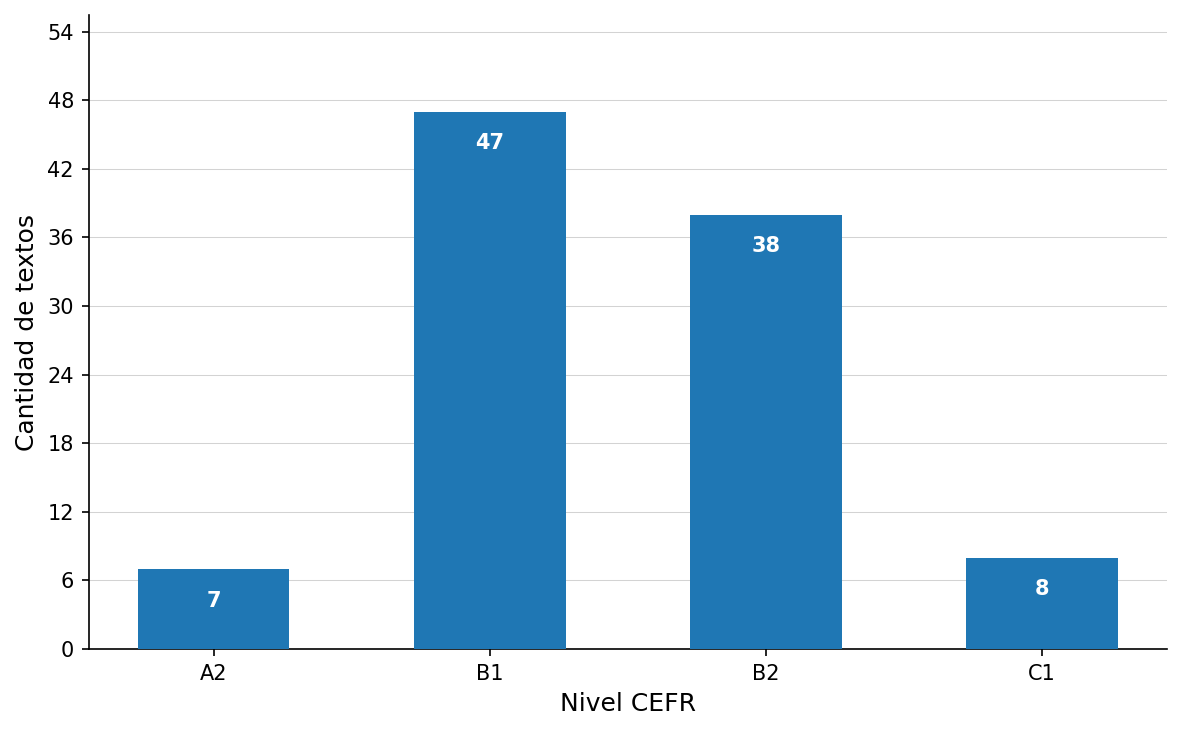
\includegraphics[width=\linewidth]{Graficos_Tesis/distribucion_cefr_originales.png} 
  \caption{Distribución de los niveles CEFR asignados por el clasificador de la competencia TSAR a los fragmentos de texto originales sin adaptar.}
  \label{fig:distribucion}
\end{figure}

\subsubsection{El dilema entre adecuación de nivel y preservación del significado}

A partir de los experimentos realizados, se hace evidente la existencia de un relación de compromiso entre la precisión en la adecuación al nivel CEFR objetivo y la fidelidad semántica respecto al texto original.

En nuestras pruebas, las estrategias que forzaban una simplificación más agresiva para cumplir con los descriptores de los niveles A2 o B1 tendían a incurrir en omisiones de información crítica o en la pérdida de matices argumentativos. Por el contrario, los sistemas que priorizaban la preservación del significado (como el Run 3) a menudo mantenían estructuras o términos que los clasificadores automáticos interpretaban como superiores al nivel objetivo.

Este fenómeno puede atribuirse a tres factores:
\begin{enumerate}
\item \textbf{Capacidad del modelo:} Las limitaciones de los modelos de 8B para realizar paráfrasis complejas que reduzcan la sintaxis sin sacrificar el contenido.
\item \textbf{Discordancia de métricas:} La falta de alineación entre las métricas de similitud semántica (como \textit{MeaningBERT}) y los criterios de legibilidad, especialmente en el nivel B1, donde los límites entre niveles son difusos  y dependen de interpretaciones pedagógicas sutiles.
\item \textbf{Naturaleza de la tarea:} La simplificación controlada es intrínsecamente más difícil que la clasificación, ya que requiere un equilibrio perfecto entre la reducción lingüística y la integridad del mensaje.
\end{enumerate}

\subsubsection{Benchmarking: Desempeño relativo frente al estado del arte}

Para situar los resultados de \textit{TaskGen} en el contexto de la competencia, es necesario analizar las estrategias de los equipos que ocuparon las primeras posiciones del ranking:

\begin{itemize}
\item \textbf{EhiMeNLP (1º puesto):} Implementaron una estrategia de dos pasos basada en la generación de múltiples adaptaciones mediante diversos modelos (GPT-5, GPT-4.1, O3, gpt-oss-20b, Llama-3.3-70B-Instruct y Qwen3-32B) y una variedad de prompts. Su flujo de trabajo consistió en un primer ranking basado en el script de evaluación oficial, seguido de un segundo filtrado de las mejores opciones utilizando \textit{MeaningScore} y \textit{BERTScore}.

\item \textbf{UoL-UPF (2º puesto):} Su propuesta se centró en maximizar la similitud semántica con la referencia humana. Generaron múltiples variantes variando prompts e intentos con modelos como GPT-4.1-mini, gpt-oss-20b, Gemma-3-4b-it y Qwen-2.5-14b-it. Aplicaron filtros de nivel CEFR y \textit{meaning score} para finalmente seleccionar la salida óptima mediante un criterio de \textit{Minimum Bayes Risk} (MBR) [cita].

\item \textbf{HIT-YOU (3º puesto):} Presentaron dos enfoques distintos. El primero consistió en la generación de multiples simplificaciones filtradas por nivel CEFR y evaluadas por un LLM actuando como juez. El segundo fue un sistema iterativo donde un LLM generaba una versión que luego era clasificada; si el nivel no era el objetivo, el modelo recibía instrucciones correctivas para reescribir el texto hasta satisfacer la condición. Emplearon modelos de alta capacidad como Claude 4 Sonnet, Gemini 2.5 Flash, GPT-5 y o1.

\item \textbf{Uniandes (4º puesto):} Desarrollaron una estrategia iterativa basada en agentes. El proceso iniciaba con un preprocesamiento para la extracción y clasificación de palabras clave; posteriormente, un agente de escritura simplificaba el texto. Un agente evaluador calculaba métricas y verificaba el cumplimiento de las condiciones pedagógicas, reiniciando el ciclo en caso negativo. Utilizaron modelos como Gemini 2.5 Pro, Gemini 2.5 Flash y GPT-OSS-120B.

\item \textbf{Archaeology (5º puesto):} Aplicaron una estrategia iterativa de generación y evaluación CEFR. Como nota distintiva, además de usar Claude Sonnet 4 y LLaMA 3.1 8B Instruct, realizaron un \textit{fine-tuning} específico para simplificación sobre el modelo LLaMA 3.2 1B utilizando datos sintéticos. Resulta relevante observar que, aunque su entrega con Claude Sonnet 4 superó a nuestro sistema, la \textit{run 3} de \textit{TaskGen} obtuvo mejores resultados que la estrategia iterativa de este equipo cuando utilizó el mismo modelo base (LLaMA 3.1 8B).
\end{itemize}

El análisis comparativo revela que las estrategias adoptadas por los equipos líderes guardan similitudes conceptuales con las planteadas en este trabajo, especialmente en el uso de arquitecturas multi-etapa y procesos de refinamiento. Un hallazgo significativo es que la mayoría de estos sistemas dependieron de modelos privativos de última generación o modelos abiertos de gran escala (superiores a 70B parámetros).

En este contexto, el desempeño de \textit{TaskGen} valida la efectividad de la arquitectura de \textit{ensemble} por votación y el uso de recursos lingüísticos explícitos. Los resultados demuestran que es posible alcanzar niveles de calidad competitivos utilizando modelos de parámetros reducidos (8B), los cuales, mediante un diseño de prompts robusto, logran equipararse en diversas métricas a modelos de mayor envergadura.

\subsection{Conclusiones}\label{sec:ad_conclusiones}

El trabajo presentado en este capítulo permite extraer conclusiones significativas sobre la viabilidad y eficacia de los LLMs de parámetros reducidos en la tarea de simplificación controlada por niveles de legibilidad (RCTS). A través de la experimentación con el sistema \textit{TaskGen}, se ha validado que la arquitectura de \textit{ensemble} por votación heurística (\textbf{Run 3}) constituye la estrategia más robusta, logrando un equilibrio superior entre la fidelidad semántica y la adecuación pedagógica.

Los resultados obtenidos en la \textit{shared task} TSAR 2025 sitúan a nuestra propuesta en una posición competitiva frente al estado del arte, destacando especialmente en la preservación del significado respecto al texto original (0,856) y a las referencias expertas (0,826). Es particularmente relevante el hecho de que un modelo de 8 mil millones de parámetros, potenciado por un diseño de \textit{prompts} enriquecidos con recursos lingüísticos explícitos, haya logrado superar a estrategias iterativas de otros equipos basadas en el mismo modelo base, e incluso equipararse en rendimiento a sistemas que emplearon modelos privativos de mayor escala. Esto confirma que el esfuerzo en ingeniería de \textit{prompts} y la incorporación de descriptores CEFR y listas de vocabulario graduado compensan, en gran medida, las limitaciones de tamaño del modelo.

No obstante, la investigación también ha revelado desafíos metodológicos y técnicos críticos:
\begin{itemize}
\item \textbf{La brecha entre niveles:} Se observó una dificultad significativamente mayor para adaptar textos hacia el nivel B1 en comparación con el nivel A2. Esto sugiere que las fronteras lingüísticas en niveles intermedios son más difusas y requieren de un control sintáctico más fino que el proporcionado por instrucciones directas.
\item \textbf{El compromiso entre métricas:} Existe una tensión inherente entre simplificar el lenguaje para cumplir con un nivel bajo de CEFR y mantener la integridad del mensaje. Una simplificación agresiva suele derivar en la pérdida de matices argumentativos, mientras que una alta fidelidad semántica tiende a mantener la complejidad por encima del umbral objetivo.
\item \textbf{Sesgo del corpus:} La fragmentación de los pasajes originales del British Council para conformar el \textit{dataset} de evaluación introduce una ambigüedad en la clasificación de niveles, lo que indica que la contextualización del texto es un factor clave que los modelos y evaluadores automáticos deben considerar.
\end{itemize}

\subsection{Trabajo futuro}
Como trabajo futuro, nos proponemos profundizar en la contribución específica de cada componente lingüístico del \textit{prompt} (descriptores vs. listas de palabras vs. estructuras morfosintácticas) para aislar su impacto individual en el desempeño del modelo. Asimismo, planeamos optimizar la heurística de votación mediante el ajuste de pesos derivados de datos empíricos en lugar de criterios manuales, para lo cual se trabajará en la expansión del corpus etiquetado.

Finalmente, se explorarán estrategias de \textit{prompting} más avanzadas, incluyendo arquitecturas de agentes en paralelo donde ramas separadas se especialicen en la adecuación CEFR y la fidelidad semántica antes de una síntesis final. Por último, se proyectan experimentos de ajuste fino (\textit{fine-tuning}) guiados por métricas de evaluación automática, buscando armonizar definitivamente la preservación del significado con las restricciones de legibilidad pedagógica.
